Ground is composed of a foundational metamodel and the sub-services that back it up.  The metamodel and its Northbound API are critical: they define the Ground surface and semantics, reflecting the new data practices we wish to capture and enhance.  Metamodel definition and support represents the first code we are writing for Ground, and we expect to continue to maintain and evolve it over time.  Behind the metamodel is the Southbound API to five basic services described below.  

We are currently in the midst of an agile development cycle, building and releasing a Minimum Viable Prototype (MVP) of Ground that we call \emph{Ground Zero}. Where appropriate we describe our goals and status for the MVP separately from the longer-term discussion.  A sketch of the Ground Zero architecture is provided in Figure~\ref{fig:layers}.

\begin{figure}
\centering
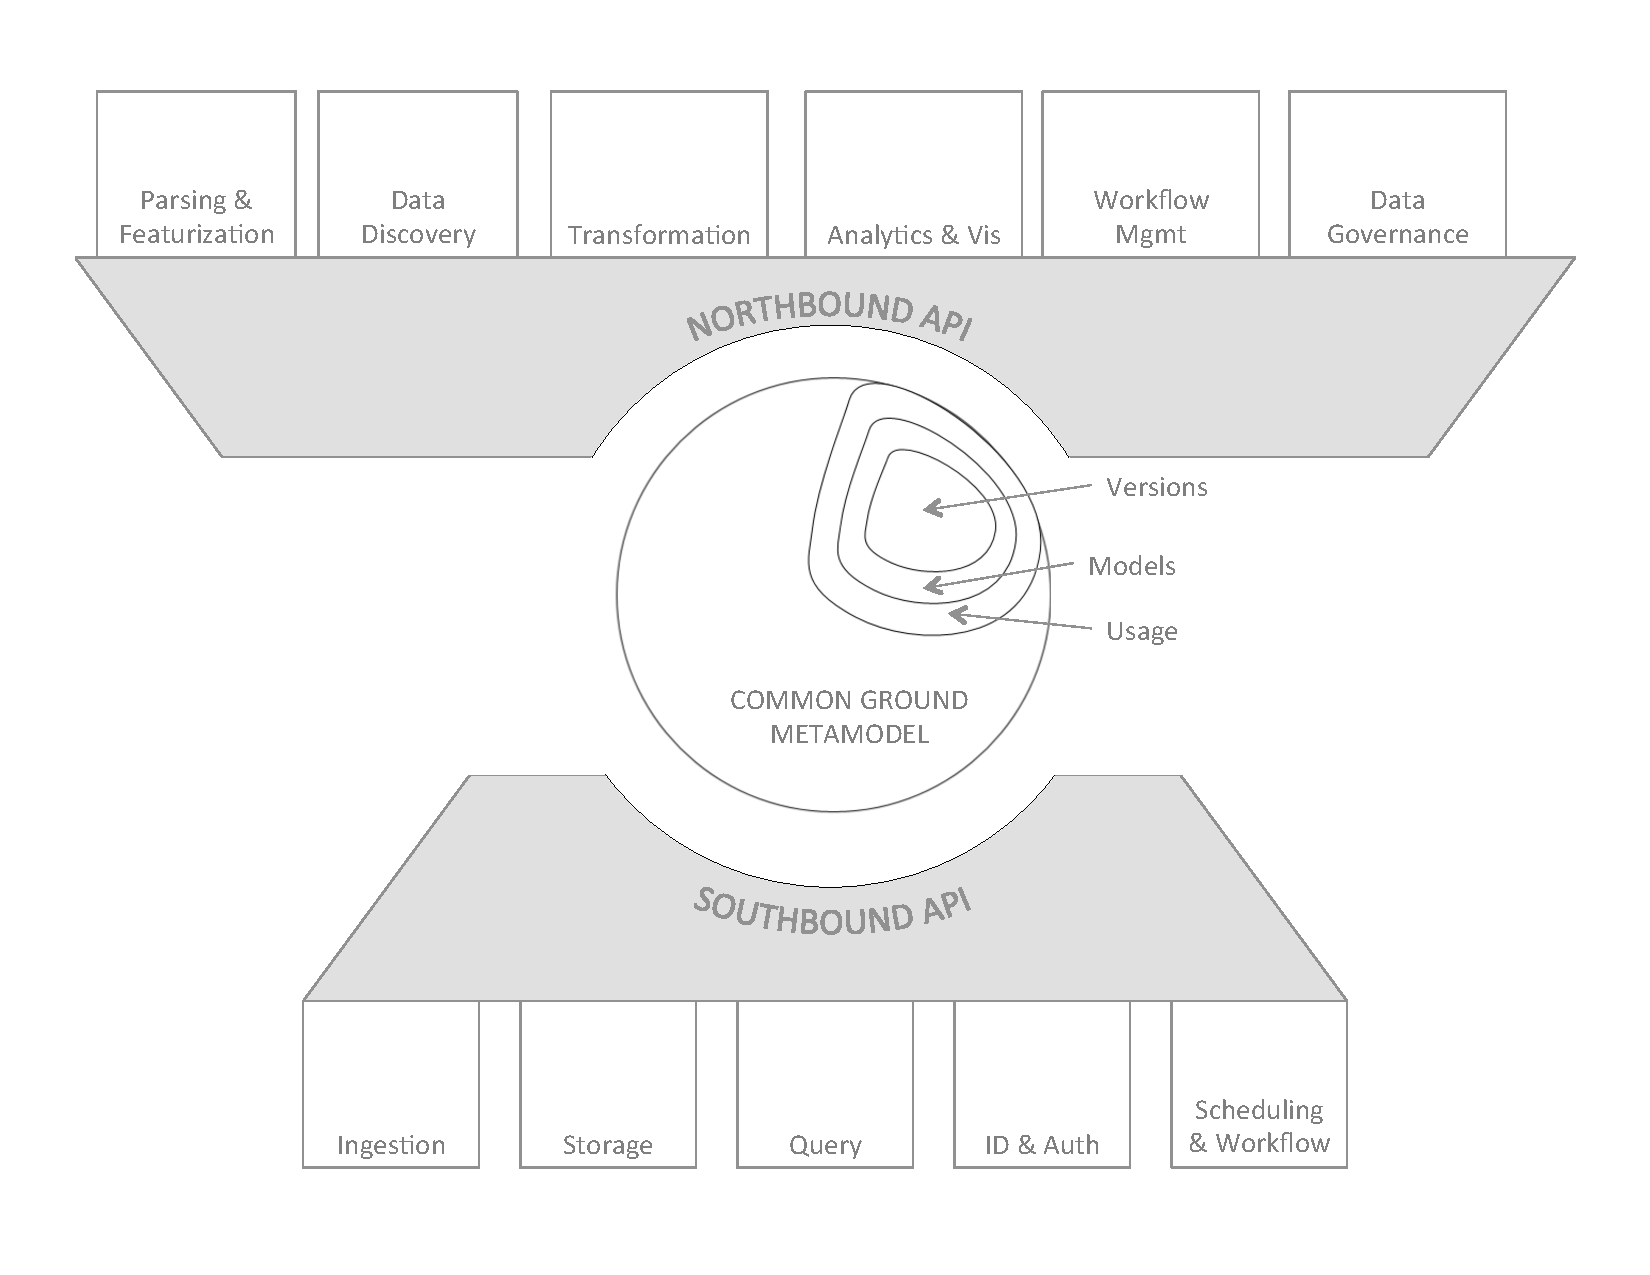
\includegraphics[width=0.75\linewidth]{ground0fig.pdf}
\caption{A sketch of the Ground architecture.}
\label{fig:layers}
\end{figure}

\subsection{The Common Ground Metamodel, In Brief}


We begin with an overview of our metamodel, \emph{Common Ground}, which is described in detail in a companion document~\cite{ground-metamodel}; we provide an overview here.  Common Ground provides a three-layer metamodel, with three intertwined graphs capturing versioning at the \emph{core} of the model, metadata modeling at the intermediate \emph{mantle} level, and usage information at the outer \emph{crust} layer.  The core versioning model supports arbitrary DAGs of versions that can be managed in Ground, or be shadowed from external versioning systems like Git. All metadata in Ground is intrinsically versioned. The mantle modeling layer offers an inclusive graph representation that can capture metadata that is represented in both structured and unstructured forms side-by-side, subsuming standard models like Relational, JSON documents, key-value stores and XML.  Usage logs, principals and lineage DAGs in the crust are the third key aspect of the metamodel, enabling the tracking of lineage across both nodes and edges in the underlying models.  The interested reader is referred to the Common Ground design document~\cite{ground-metamodel} for more detail.

A prototype implementation of Common Ground has been implemented in Scala and is in active use in a deployment at UC Berkeley managing metadata for a large undergraduate course on Database Systems with 500 students and 10 staff. It is tracking metadata about user identity across three authorization systems at Berkeley, workflows and scripts in Python, SQL, PySpark and Jupyter Notebooks, and code versioned externally at GitHub.  This prototype of the metamodel forms the initial basis of the Ground Zero MVP, and has driven the prototypes of some of the services described next.

\subsection{Key Services}
Ground's functionality is backed by five key sub-services.  It was our goal for the initial Ground Zero prototype to use existing open source solutions where possible.  We expect that some of these solutions will fail, and that innovative research will be required to develop viable technology for these services at scale.

\begin{enumerate}
\item \textbf{Versioned Metadata Storage}.  Ground must work with storage in two senses: it must store versioned metadata reliably, and manage references to externally stored data as well.  Ground must be able to store metadata with the full richness of the Common Ground metamodel, including flexible version management, data modeling and lineage storage.  Ground also needs to reference external data, which can come in arbitrary form, with a wide variety of APIs.  Note that Ground is not the primary interface for accessing the data that is referenced by metadata; Ground is expected to \emph{describe} external data and track it, not serve it.  Hence Ground's most basic requirement for external data is to know how to store a unique ID for each item it tracks, and return that ID to applications that request it.  In an ideal setting, each external data item is versioned, hence each version has a unique ID.  However if the external item is mutable and not versioned, Ground generates \emph{Schr\"{o}dinger versions} lazily: each time we observe an object we assume it changes, and assign it a new version (and version ID).  This is discussed in more detail in the Common Ground design~\cite{ground-metamodel}.

\textbf{MVP:} We are currently mapping our metadata model onto a traditional PostgreSQL relational database for storage.  Graphs can be represented as relations, so we manage versions, lineage and data modeling graphs at application level above the relational model.  PostgreSQL is a fairly mature system but is not designed to meet our requirements for latency, scalability and availability. In fact we do not expect any relational solution to work well for our needs over time, as relational databases are not designed for any of the three key individual aspects of the metamodel: versioned data, polyglot data models, or rich lineage.  Unfortunately, we do not expect that solutions in the NoSQL or graph database world will fare well either, though this requires research to validate. Therefore a critical thrust of the Ground research agenda is to understand the weaknesses of existing database systems when faced with these requirements, and design a new database system that is well-suited to emerging metadata workloads. \jmh{Need to call out research hypotheses more clearly.}


\item \textbf{Search, Query, Analyze}.  As noted above, Ground is intended to be permissive in the kind of metadata it stores.  First, it needs to support a least-common denominator of unstructured tags, and provide efficient search over those tags.  To this end it needs an indexing and search component.  Second, Ground also needs to support efficient interactive behavior for applications that are inserting, updating and fetching metadata---and capture any changes in a versioned manner.  This should be provided by the metadata storage service with low latency and high throughput.  Third, we expect that metadata will produce a rich target for analytical workloads: algorithms that study what data exists over time, as well as who, how and why data gets used and gets changed.  Finally, it seems natural that some workloads will need to combine these three classes of queries, perhaps via a federated query layer above them. 

\textbf{MVP:} Initially we are not supporting search or analytic APIs; these will be added as the system evolves.  For interactive query, we can only do as well as our prototype relational metadata store.  For search, we expect that existing solutions like Solr will be sufficient for the foreseeable future; we do not expect metadata tagging and querying to exceed volumes that Solr sees in free-text indexing. For analytics, we intend to leverage Spark and GraphX as we have significant expertise in house.  However, the nature of the analytics to be done here represents a major research opportunity: what might be the value of metadata in a Big Data context, and how could that value be extracted by analytics?  Could a \emph{self-aware} Big Data ecosystem improve itself, or provide valuable insight about its usage to applications and users?  \jmh{Again, call out research.}  Finally, the requirements for a federated query layer and its design are a topic for investigation after we acquire a corpus of metadata and workloads.

\item \textbf{Ingestion: Insertion, Queues and Crawlers}.  Metadata may arrive to be stored in Ground interactively or in batches, and it may come actively (via a ``push'' insertion interface), or passively (via a ``pull'' crawling interface).  Interactive insertion of metadata needs to be supported efficiently by the metadata storage component; batch insertion should make use of queueing services to handle bulk delivery and bursty arrivals.  Passive insertion needs to be handled via a data crawler that can register metadata from external services with Ground, and see if Ground can enrich that metadata via additional software services for file parsing and feature extraction.

\textbf{MVP:}  Currently we are handling ingest solely via simple push insertion APIs that call into our metadata store via SQL.  However we envision integrating open-source solutions like Kafka for queuing, and Gobblin for crawling and data ingest from remote sources.  We are also eager to explore APIs to plug in third-party solutions for  extracting metadata from crawled data; two examples we are OpenCalais (a free automated service for entity extraction) and Trifacta (a commercial, semi-automatic solution for data transformation).  We also recognize that there are boundless R\&D opportunities here, some of which could be part of Ground, many of which should exist as standalone solutions above Ground.  \jmh{another research opening, though more about opportunities above ground.}  We look forward to integration with other research and non-research colleagues here.

\item \textbf{Identity and Authorization Integration}.  Identity management and authorization are a required aspect of the Ground service, but almost certainly one that we want to delegate if we can.  The primary reason not to ``bake in'' authorization is administrative: most organizations already have an authorization service and do not want their metadata service to impose a new one.  More importantly, authorization is a semantic notion with wide flexibility: the authorization policies of a federal defense agency are likely to be wildly different in nature from those of a marketing department doing targeted advertising, or an international consortium of scientists interested in reproducibility.  The flexible design of Ground's metamodel should make it possible for a wide variety of use cases to capture authorization metadata (ownership, auditing, content labeling etc.) and design policy over that metadata.  An open design question is whether Ground needs to \emph{enforce} policy, or merely store it.  Note that there is a subtle set of multidimensional connections between metadata versions and policy versions, particularly when the aurthorization policies of a past time are considered unsafe later---a case where good people may disagree about the virtues of immutability.

\textbf{MVP:}  The current MVP has no support for identity management and authorization.  However our initial use case has us tracking UC Berkeley student IDs, Github identities, UNIX uids from instructional computing, and associations between the three; visibility of things like grading scripts and their outputs will depend on policies regarding these identities.  In the short term we expect to integrate with Google oAuth services as exposed at UC Berkeley next, and to explore the way that policy is specified and possibly enforced in our prototpype environment.  Our longterm roadmap here remains open; we expect a need to collaborate closely with partners in application domains to get further requirements.  \jmh{Possible tie to Raluca's work here, at minimum as an example of a non-standard approach to these issues.}

\item \textbf{Scheduling, Workflow, Reproducibility}. In this domain, it is important to separate specification from execution.  We are committed to ensure that Ground is flexible and rich enough to capture the specification of workflows at many granularities of detail: from black-box executables to workflow graphs to source code.  However, we do not expect Ground to be a universal provider of workflow execution or scheduling; instead we hope to integrate with a variety of schedulers and execution frameworks including on-premises and cloud-hosted approaches.

\textbf{MVP:} We plan to begin by utilizing the scheduling and execution services provided by the Gobblin project, which supports a variety of schedulers including Quartz, Azkaban and Oozie, and execution frameworks including Yarn and Helix.  We plan to look into support for VMs and containers as well.  \jmh{Certainly could paint a research picture here, closer to the Bloom-meets-Kubernetes agenda: how will data-centric workflows be programmed in the future, especially as we look at containers, elastic services, etc?}  maybe also a connection to the Shenker/Jackson work on Declarative Datacenters?
\end{enumerate}